%************************************************
%\chapter{Image Preprocessing}\label{ch:preprocessing} % 
\chapter{General Methodology}\label{ch:preprocessing} % $\mathbb{ZNR}$
%************************************************
To perform most automated analyses on neuroimaging, it is fundamental that images are comparable. Preprocessing comprises a series of algorithms that, applied after the acquisition and reconstruction of the images, produce directly comparable images in both structure and magnitude. 

In this section we present the preprocessing algorithms used in this thesis. Whether they have been used in one or all experiments, they can be classified in two major categories: spatial and intensity preprocessing. Later, in Section~\ref{sec:vwanalyses}, we present some voxelwise analyses, commonly used in clinical practice, that we have set as a baseline in our experiments. 

\section{Spatial Preprocessing }
Spatial processing usually accounts for the differences in position, angles and structure that are commonly found between images. A common pipeline in, for example, \ac{MRI} preprocessing, is the one found at Figure~\ref{fig:examplePreMRI}, where the images are registered (or spatially normalized) to a template, smoothed and finally segmented. The smoothing is an optional step, generally used in procedures like segmentation or \ac{VBM}. 

\begin{figure}[htp]
	\myfloatalign
	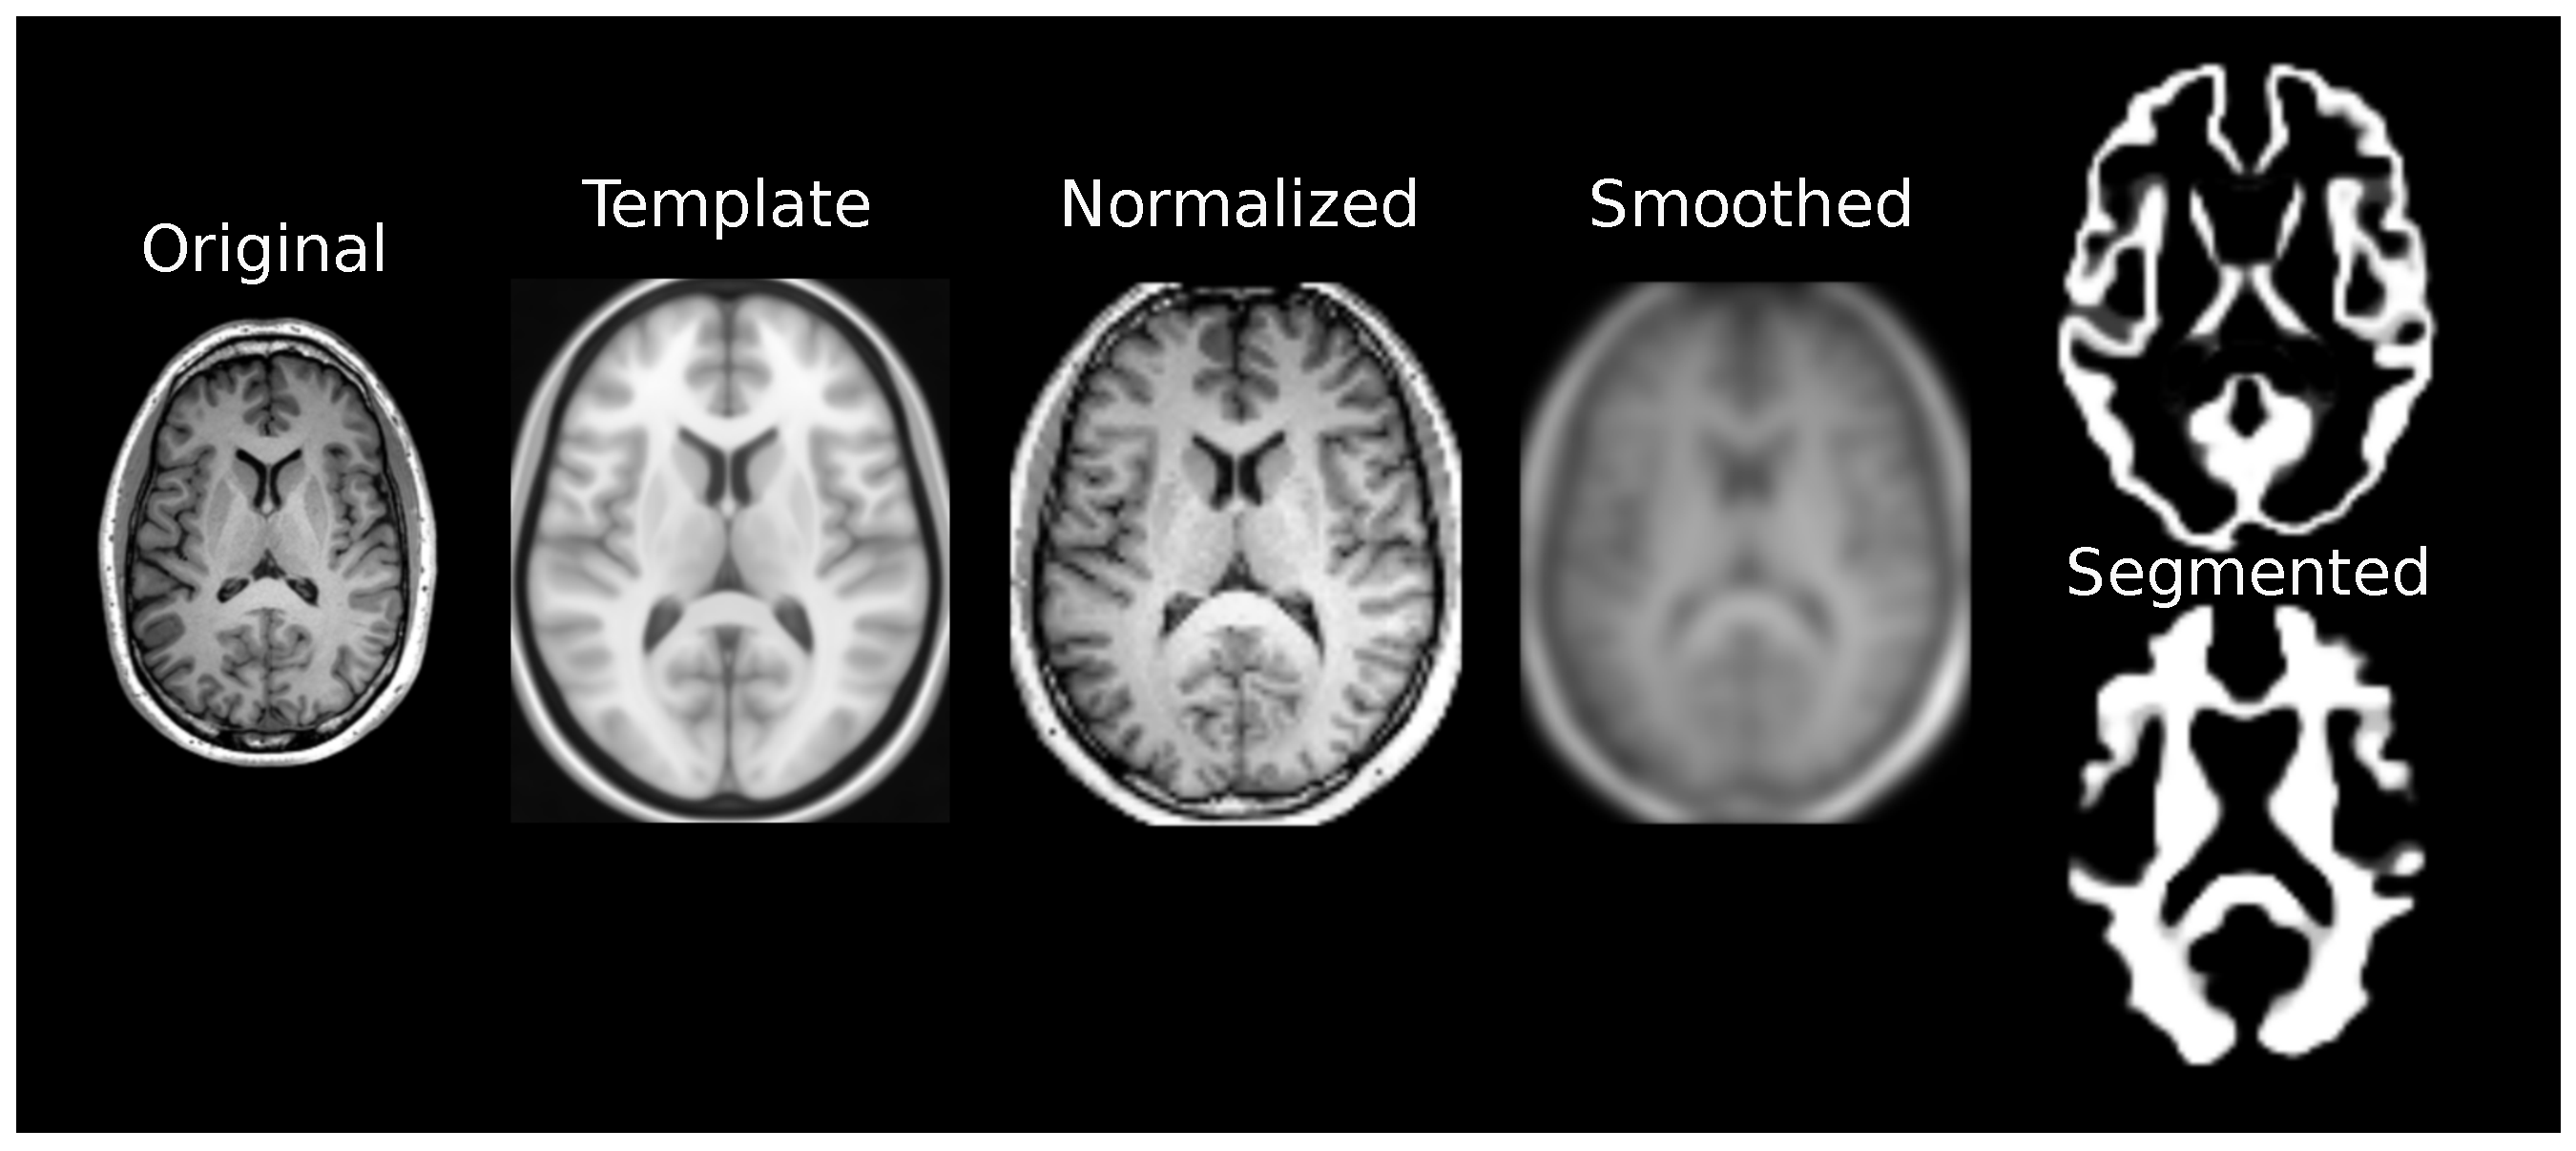
\includegraphics[width=.75\linewidth]{Graphics/ch3/preProcessPL}
	\caption[Typical pre-processing pipeline in MRI]{Typical pre-processing pipeline in \ac{MRI}.}\label{fig:examplePreMRI}
\end{figure}

In this thesis, all the experiments in all image modalities involve spatial normalization. Smoothing, as well as segmentation, is only applied in some experiments that use \ac{MRI} images, such as the segmented images in Chapter~\ref{ch:sbm} or the whole-brain analysis performed in Chapter~\ref{ch:swpca}. 

\subsection{Spatial Normalization or Registration}
Spatial Normalization, also known as Registration, is the procedure that by which every subject's brain is mapped from their individual space to a standard reference system. Registered images allows our system to overcome the individual differences in position and anatomy by establishing a common reference space in which a given coordinate represent the same anatomical position in all brains in the dataset. 

There exist a number of pieces of software widely used for registering images, such as FreeSurfer \cite{Reuter2010} or FSL (in the FLIRT and FNIRT package) \cite{Smith2004}, most of them perform linear, non-rigid and elastic transformations or a combination of these. In this work we have used the software SPM8 \cite{spm_book} to perform registration of all the datasets, including \ac{MRI}, \ac{SPECT} and \ac{PET} images. So, from this moment, we will focus on the registration as performed in the \ac{SPM8}. 

Linear registration usually refers to the affine transformation, a matrix multiplication that includes 12 parameters for translation, rotation, scale, squeeze, shear and others: 
\begin{equation}\label{eq:affine}
	\left[\begin{matrix}
	x'\\y'\\z'\\1
	\end{matrix}\right]
	 = \left[\begin{matrix}
	 a_{00} & a_{01} & a_{02} & a_{03}\\
	 a_{10} & a_{11} & a_{12} & a_{13}\\
	 a_{20} & a_{21} & a_{22} & a_{23}\\
	 0 & 0 & 0 & 1\\
	 \end{matrix}\right]
	 \left[\begin{matrix}
	 x\\y\\z\\1
	 \end{matrix}\right]
\end{equation}

This matrix multiplication is performed globally, as it transforms the whole image, not accounting for local geometric differences. In equations \ref{eq:affine1}, \ref{eq:affine2} and \ref{eq:affine3} we give an example of the parameters that are computed for scale, translation and shear in 3D:

\begin{align}
\label{eq:affine1}
	\text{scale} &= 
	\left[\begin{matrix}
		 s_x  &0 & 0 & 0\\
		0 &s_y &0 &0\\
		0 &0 &s_z &0\\
		0 &0 &0 &1		
	\end{matrix}
	\right]\\
	\label{eq:affine2}
	\text{translation} &= 
	\left[
	\begin{matrix}
	1  &0 & 0 & \Delta x\\
	0 &1 &0 &\Delta y\\
	0 &0 &1 &\Delta z\\
	0 &0 &0 &1		
	\end{matrix}
	\right] \\
	\label{eq:affine3}
	\text{shear} &= 
	\left[\begin{matrix}
	1  &h_{xy}& h_{xz} & 0\\
	h_{yx} &1 &h_{yz} &0\\
	h_{zx} &h_{zy} &1 &0\\
	0 &0 &0 &1		
	\end{matrix}
	\right]
\end{align}

The combination of all these operations result in the estimation of the twelve parameters that we found in Eq.~\ref{eq:affine}, which are the ones used in \ac{SPM8}. The estimation of these parameters is performed via the optimization of a cost function, that in \ac{SPM8} can be the minimum squared difference between the source image and the template \cite{spm_book} in the case of within-modality registration, or the mutual information in between-modality registration. These functions are also used in FLIRT \cite{Jenkinson2001}, whereas FreeSurfer uses the Tukey's biweight function (in {\ttfamily mri\_robust\_template}) \cite{Reuter2012}.

After the affine transform, the software usually performs a fine-tuning step via nonrigid transformations, to account for relevant a\-na\-to\-mi\-cal differences between subjects. Nonrigid transformations range from the use of radial basis functions, physical continuum models and the large deformation models, or diffeomorphisms, that \ac{SPM8} uses. These procedures work by estimating a warp-field and then, apply it to the affine-registered images. An example of the differences of using only affine registration and applying diffeomorphisms can be found at Figure~\ref{fig:diffeomorphisms}.

\begin{figure}[bth]
	\myfloatalign
	\subfloat[Comparison in \ac{MRI}.]
	{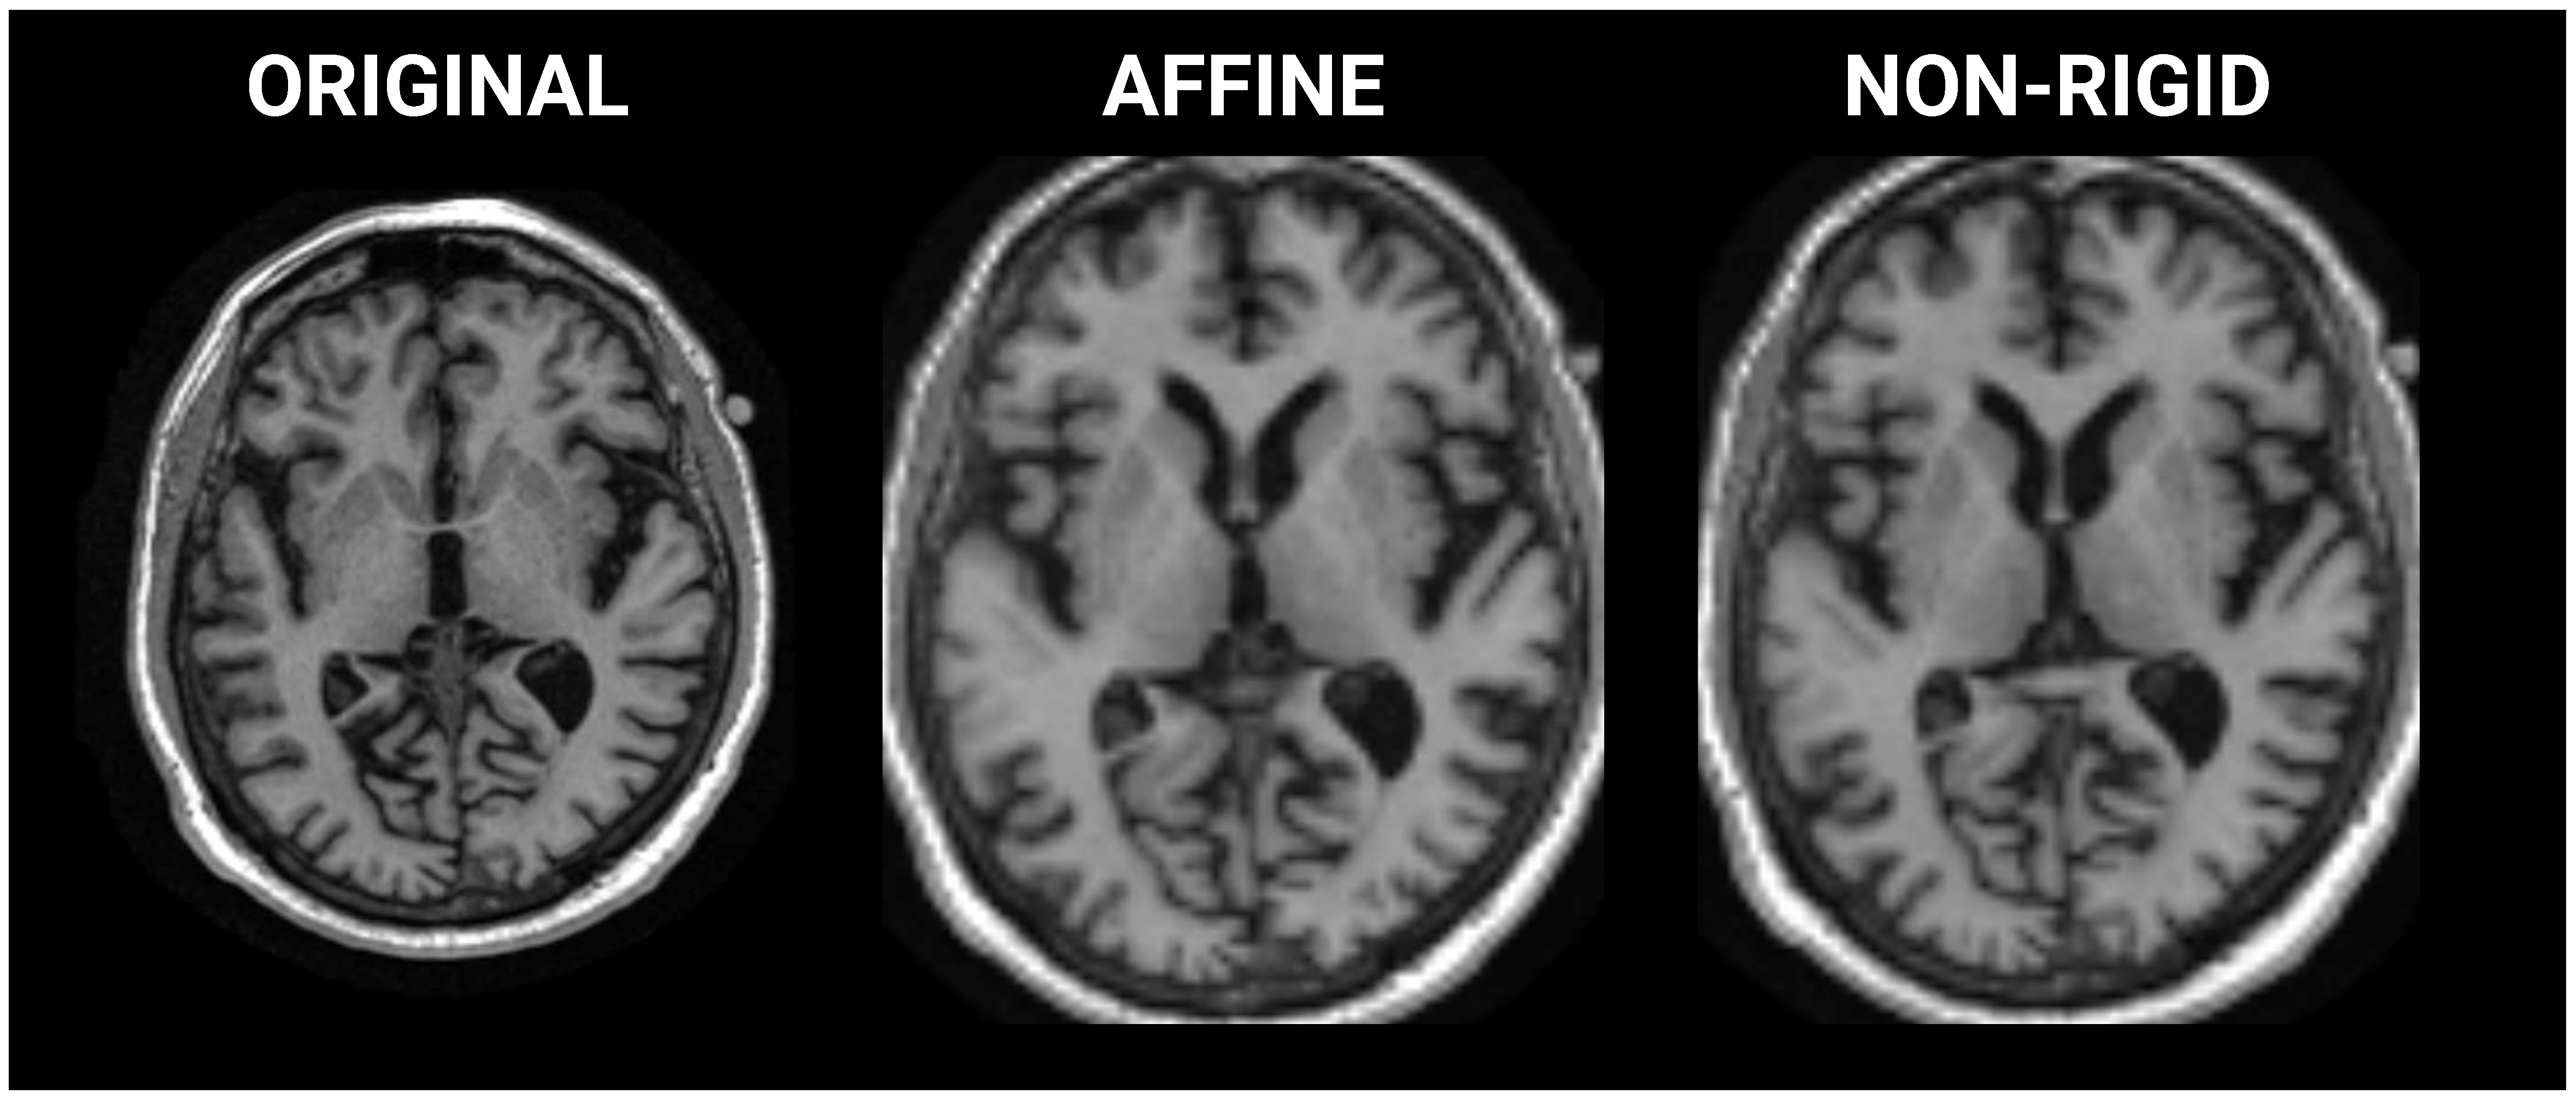
\includegraphics[width=.7\linewidth]{Graphics/ch3/regComparisonMRI}}
	 \\
	\subfloat[Comparison in \ac{PET}.]
	{\includegraphics[width=.7\linewidth]{Graphics/ch3/regComparisonPET}}
	\caption[Comparison of the affine registration and the application of non-linear transformations to the images]{Comparison of the affine registration and the application of non-linear transformations to both \ac{MRI} and \ac{PET} images of the same \ac{ADNI} subject.}\label{fig:diffeomorphisms}
\end{figure}


\subsubsection{Co-registration}
Sometimes we have several image modalities of the same subject, for example \ac{MRI} and \ac{PET} or functional \ac{MRI}, often acquired at the same time. In this particular case, we can use the higher resolution \ac{MRI} image to calculate the affine parameters and warping, and apply those to all modalities of the same subject. To do so, we perform a first co-registration, that is, a registration of the lower-resolution images (e.g. \ac{PET}) to its correspondent \ac{MRI} image. Being anatomically similar, the co-registration usually comprises a single affine transformation. Afterwards, we can proceed with the registration of that \ac{MRI} image to the template, and apply the same transformation to all its co-registered images. 

\subsubsection{The MNI Space}
In this thesis, all images are coregistered to the \acf{MNI} space \cite{Mazziotta2001}. This is the most widely used coordinate system, recently adopted by the International Consortium for Brain Mapping (ICBM) as its standard template. The three-dimensional coordinate system defined in \ac{MNI} was intended to replace the Tailarach space, a system based on a dissected brain, that was used to compose an atlas by Tailarach and Tournoux \cite{Talairach1988c}. The current template is known as ICBM152, and features the average of 152 normal \ac{MRI} scans matched to an older \ac{MNI} template using a nine parameter affine registration. 

\subsection{Segmentation}
When using \ac{MRI} images in this thesis, we often refer to \acf{GM} and \acf{WM} maps, which is the result of the segmentation of the original data. Segmentation aims at producing maps of the distribution of different tissues, and it generally addresses \ac{GM}, \ac{WM} and \ac{CSF} classes, although lately some software can output data for bone, soft tissue or very detailed functional regions and subregions \cite{Fischl2002}. 

In this thesis we have used the \ac{VBM} toolbox of the \ac{SPM8} software, which yields \ac{GM}, \ac{WM} and \ac{CSF} maps. It features an \ac{EM} algorithm to model the distribution of the tissue classes as a mixture of gaussians and, by combining this distribution-based information with tissue probability maps using a bayesian rule, the software produces joint posterior probability maps for each tissue. To clean up the segmentation maps, a series of iterative dilations and erosions are used. Finally, since brain regions are expanded or contracted at the spatial normalization step, we can scale the segmented maps using modulation, producing final maps where the total amount of grey matter is preserved. 

\section{Intensity Normalization}
Generally, structural modalities such as T1 and T2-weighted images are considered unitless, in contrast to functional imaging, in which each voxel's intensity represent the distribution of some biomarker, such as glucose metabolism, dopamine transporters, etc. These amounts are affected by many sources of variability that can affect the final values: contrast uptake, radiotracer decay time, metabolism, etc. Therefore, along with the previous spatial normalization, there is a need to normalize the intensities of the images, so that the amount they represent are comparable. 

In the case of intensity normalization, the method acts as a linear transformation of the image, preserving fundamental information such as contrast between regions. This approximation estimates the new intensity values $I'$ as: 
\begin{equation}
	I' = I/I_p 
\end{equation}
where $I_p$ is a constant parameter that is unique for each image. After this division, the new intensities would be directly comparable. The technique used to compute the normalization parameter varies, ranging from the simplest normalization to the maximum \cite{Salas-Gonzalez2009,Martinez-Murcia20129676} to complex methodologies that use assumptions about the image's \ac{PDF}. 

The \emph{normalization to the maximum} strategy computes $I_p$ as the average value of the 95th bin of the histogram of the image. In other words, this mean averaging the 5\% higher intensity values and use this mean as $I_p$. Another useful approach is the so-called \emph{integral normalization}, which computes $I_p$ as the sum of all values in the image. 

Other approaches involves some a-priori knowledge about the intensity distribution of normal subjects in a certain modality. This is the case of setting $I_p$ to the Binding Potential (BP), a ratio between the intensities at specific and non-specific areas \cite{Scherfler2005}. 

Finally, more advanced approaches use a general linear transformation of the image: 
\begin{equation}
	I' = a I + b
\end{equation}
The parameters $a$ and $b$ are so that the \ac{PDF} of a given matches a reference \ac{PDF}. There exist methods that use the histogram \cite{Arndt1996}, the gaussian distribution or the alpha-stable distribution \cite{Salas-Gonzalez2013}. In this latter case, the parameters $a$ y $b$ are computed as linear transformations of some distribution's parameters: 
\begin{equation}
	a = \frac{\gamma*}{\gamma}, \quad b = \mu* + \frac{\gamma*}{\gamma} \mu
\end{equation}
where $\gamma*$ and $\gamma$ are the dispersion parameters of the alpha-stable intensity distribution of the non-normalized and the reference image respectively, and $\mu*$ and $\mu$ are the location parameters of the same images. 

Despite traditionally structural modalities such as \ac{MRI} did not use intensity normalization, there exist a new tendency towards the use of \ac{qT1} and \ac{qT2} images \cite{Weiskopf2013} that provide biomarkers for absolute measures such as myelination, water and iron levels. This strategy is especially designed to overcome different sources of variability that affect multicentre studies, e.g. magnetic field inhomogeneity, noise, evolution of the scanners, etc. The role of those in multi-centre studies is addressed at Chapter~\ref{ch:swpca}. 

See Figure~\ref{fig:comparisonIntNorm} for a comparison between different strategies of intensity normalization on the same images. 

\begin{figure}[bth]
	\myfloatalign
	\subfloat[Normalization to the Maximum.]
	{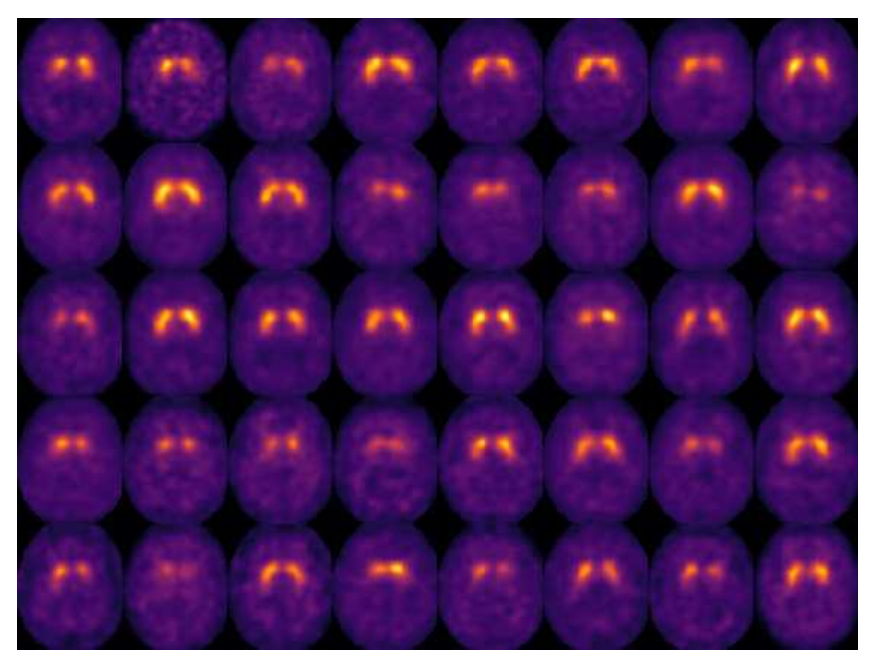
\includegraphics[width=.45\linewidth]{Graphics/ch3/norm_max.eps}}\quad
	\subfloat[Integral Normalization.]
	{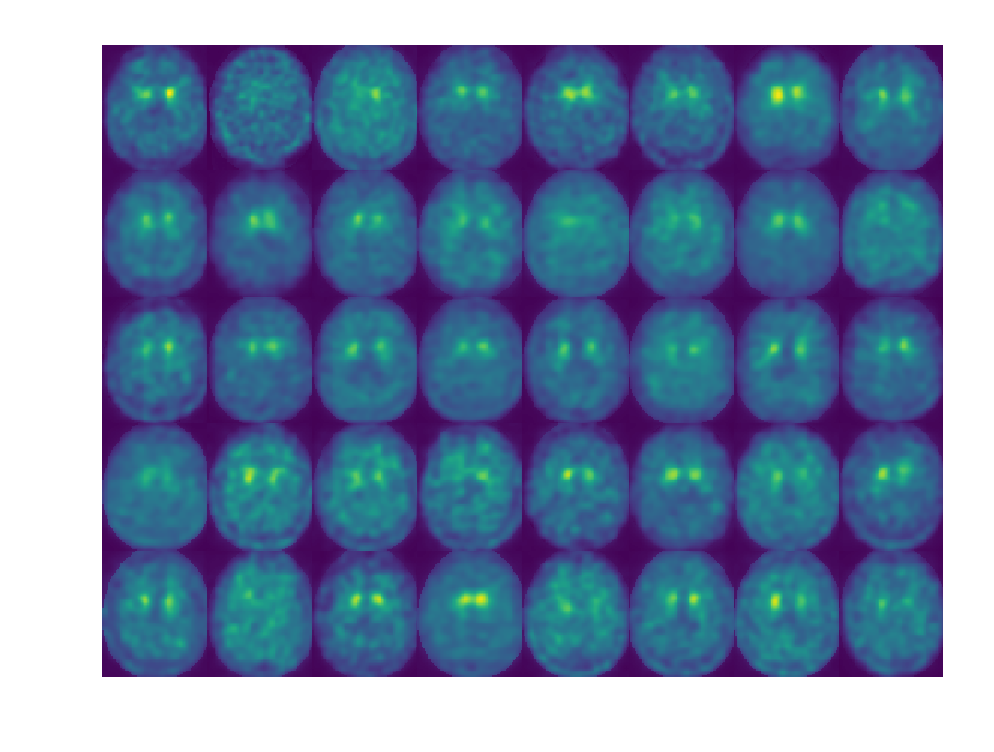
\includegraphics[width=.45\linewidth]{Graphics/ch3/norm_int.eps}}\\
	\subfloat[Normalization using $\alpha$-stable distribution.]
	{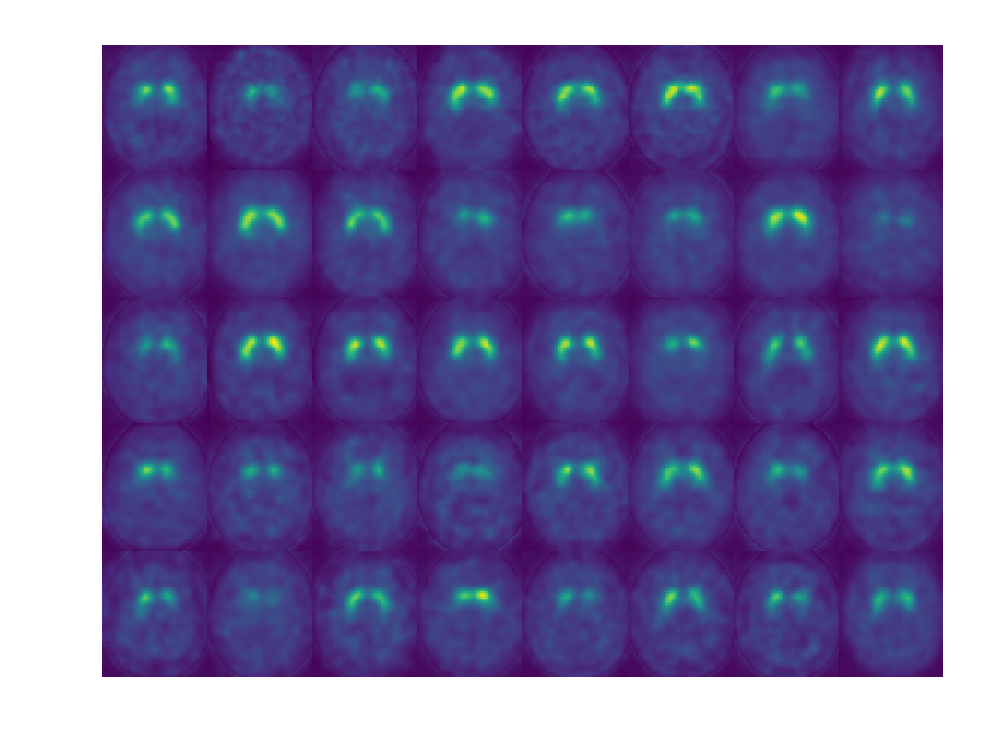
\includegraphics[width=.45\linewidth]{Graphics/ch3/norm_est.eps}}
	\caption{Comparison between different types of intensity normalization, applied to the VDLN-DAT dataset (see Appendix~\ref{ch:datasets}).}\label{fig:comparisonIntNorm}
\end{figure}
%DONE


\section{Evaluation Parameters and Methodology}\label{sec:validation}
\subsection{Cross-validation}

The classification was validated using stratified 10-fold
cross-validation (Kohavi, 1995). In brief, 9 subsets of the dataset
were used for extraction of the PCs and training of the classifier with
the remaining subset used for testing. This procedure was repeated for
each subset, repeated 10 times to avoid possible bias and random
effects of the partitions. The average and standard deviation of the
accuracy (acc), sensitivity (sens) and specificity (spec) values for
each repetition were recorded. 

\subsection{Classification Performance}

The proposed methodology has been tested on the three previously described databases, using a cross-validation method called leave-one-out to extract several performance parameters: accuracy, sensitivity, specificity, positive likelihood (PL) and negative likelihood (NL). This method achieves an almost unbiased error estimate, however it might be affected by the database topology, reason why we used different databases to test our method.

Along with the widely used sensitivity, specificity and accuracy (which are prevalence dependent), we use the Positive and Negative Likelihood ratios (PL and NL) to provide some prevalence independent parameters that are also widely used in clinical medicine, where values of PL greater than 5 or NL values less than 0.2 can be applied to the pre-test probability of a patient having the disease tested for to estimate a post-test probability of the disease state existing \cite{McGee2002}. A positive result for a test with an PL of 8 adds approximately 40\% to the pre-test probability that a patient has a specific diagnosis. 

To provide a better understanding of the accuracy distribution (mean, range, skewness), we have made use of the box plot (Fig. \ref{fig:features_acc_distances}). In these plots, the median for each group of data is indicated by the red center line, and the first and third quartiles are the edges of the blue box, which is known as the inter-quartile range (IQR). The extreme values (within 1.5 times the inter-quartile range from the upper or lower quartile) are the ends of the lines extending from the IQR. Points at a greater distance from the median than 1.5 times the IQR are plotted individually, representing potential outliers. 


